
\ifdefined\ishandout
\documentclass[11pt,english,handout]{beamer}
\else
\documentclass[11pt,english]{beamer}
\fi

%\documentclass[11pt]{beamer}
\usepackage{mathptmx}
\renewcommand{\sfdefault}{lmss}
\renewcommand{\familydefault}{\sfdefault}
\usepackage[T1]{fontenc}
\usepackage[latin9]{inputenc}
\usepackage{amsmath}
\usepackage{amssymb}
\usepackage{graphicx}
\PassOptionsToPackage{normalem}{ulem}
\usepackage{ulem}
\usepackage{caption}
\captionsetup{labelformat=empty}
\usepackage{bbm}
\usepackage{upgreek}
\usepackage{graphicx}
\setbeamertemplate{section in toc}[sections numbered]
\makeatletter
\usepackage{caption} 
\captionsetup[table]{skip=10pt}
%%%%%%%%%%%%%%%%%%%%%%%%%%%%%% Textclass specific LaTeX commands.
 % this default might be overridden by plain title style
 \newcommand\makebeamertitle{\frame{\maketitle}}%
 % (ERT) argument for the TOC
 \AtBeginDocument{%
   \let\origtableofcontents=\tableofcontents
   \def\tableofcontents{\@ifnextchar[{\origtableofcontents}{\gobbletableofcontents}}
   \def\gobbletableofcontents#1{\origtableofcontents}
 }

%%%%%%%%%%%%%%%%%%%%%%%%%%%%%% User specified LaTeX commands.
%\documentclass[presentation]{beamer}


\def\Tiny{\fontsize{7pt}{8pt}\selectfont}
\def\Normal{\fontsize{8pt}{10pt}\selectfont}

\usetheme{Madrid}
\usecolortheme{lily}
%\setbeamercovered{transparent}
\useinnertheme{rounded}


\setbeamertemplate{footline}{\hfill\Normal{\insertframenumber/\inserttotalframenumber}}
%\setbeamertemplate{footline}{}

\setbeamertemplate{navigation symbols}{}

\newenvironment{changemargin}[2]{%
\begin{list}{}{%
\setlength{\topsep}{0pt}%
\setlength{\leftmargin}{#1}%
\setlength{\rightmargin}{#2}%
\setlength{\listparindent}{\parindent}%
\setlength{\itemindent}{\parindent}%
\setlength{\parsep}{\parskip}% 
}%
\item[]}{\end{list}}

\setbeamertemplate{footline}{\hfill\insertframenumber/\inserttotalframenumber}
\setbeamertemplate{navigation symbols}{}

%\usepackage{times}  % fonts are up to you
\usepackage{graphicx}
%\usepackage{graphics}
\usepackage{epsfig}
\usepackage{bm}
\usepackage{epsf}
\usepackage{float}
\usepackage[final]{pdfpages}
\usepackage{multirow}
\usepackage{colortbl}
\usepackage{xkeyval}
%\usepackage{sgame}
%\usepackage{pst-node}
\usepackage{listings}
\usepackage{ifthen}
%\usepackage{hyperref}
\usepackage{tikz}

%\usepackage{times}  % fonts are up to you
%\usepackage{graphicx}
%\usepackage{graphics}
\usepackage{epsfig,bm,epsf,float}
\usepackage[final]{pdfpages}
\usepackage{xcolor,multirow,colortbl}
\usepackage{xkeyval}
\usepackage{verbatim}
%\usepackage{sgame}
%\usepackage{pst-node}
\usepackage{listings}
%\usepackage{handoutWithNotes}
%\pgfpagesuselayout{3 on 1 with notes}[letterpaper,border shrink=5mm]
%\pgfpagesuselayout{2 on 1 with notes landscape}[letterpaper,border shrink=5mm]
\usepackage{setspace}
\usepackage{ragged2e}

\setbeamersize{text margin left=1em,text margin right=1em} % CambridgeUS spacing if you use default instead


%\pdfmapfile{+sansmathaccent.map}

% Table formatting
\usepackage{booktabs}


% Decimal align
\usepackage{dcolumn}
\newcolumntype{d}[0]{D{.}{.}{5}}


\global\long\def\expec#1{\mathbb{E}\left[#1\right]}
\global\long\def\var#1{\mathrm{Var}\left[#1\right]}
\global\long\def\cov#1{\mathrm{Cov}\left[#1\right]}
\global\long\def\prob#1{\mathrm{Prob}\left[#1\right]}
\global\long\def\one{\mathbf{1}}
\global\long\def\diag{\operatorname{diag}}
\global\long\def\expe#1#2{\mathbb{E}_{#1}\left[#2\right]}
\DeclareMathOperator*{\plim}{\text{plim}}

%\usefonttheme[onlymath]{serif}

\usepackage{appendixnumberbeamer}
\renewcommand{\thefootnote}{}

\setbeamertemplate{footline}
        {
      \leavevmode%
   %   \hbox{%
%      \begin{beamercolorbox}[wd=\paperwidth,ht=2.25ex,dp=1ex,right]{date in head/foot}%
        %\usebeamerfont{date in head/foot}\insertshortdate{}\hspace*{2em}%
\hfill
    %turning the next line into a comment, erases the frame numbers
        \insertframenumber{}\hspace*{2ex}\vspace{1ex}

  %    \end{beamercolorbox}}%
}

\definecolor{blue}{RGB}{0, 0, 210}
\definecolor{red}{RGB}{170, 0, 0}

\makeatother

\usepackage[english]{babel}

\usepackage{tikz}
\newcommand*\circled[1]{\tikz[baseline=(char.base)]{             \node[circle,ball color=structure.fg, shade,   color=white,inner sep=1.2pt] (char) {\tiny #1};}} 

\makeatletter
\let\save@measuring@true\measuring@true
\def\measuring@true{%
  \save@measuring@true
  \def\beamer@sortzero##1{\beamer@ifnextcharospec{\beamer@sortzeroread{##1}}{}}%
  \def\beamer@sortzeroread##1<##2>{}%
  \def\beamer@finalnospec{}%
}
\makeatother



\setbeamersize{text margin left= .8em,text margin right=1em} 
\newenvironment{wideitemize}{\itemize\addtolength{\itemsep}{10pt}}{\enditemize}
\newenvironment{wideitemizeshort}{\itemize}{\enditemize}

 \newcommand{\indep}{\perp\!\!\!\!\perp} 

\begin{document}

%% Title slide
\begin{frame}[noframenumbering]{}
\vspace{0.5cm}
\title[]{Chapter 2: Probability and Statistics}
\author{Jonathan Roth}
\date{Mathematical Econometrics I \\ Brown University \\ } 
\titlepage {\small{}\ }\thispagestyle{empty} \vspace{-30pt}

\end{frame}
 
\begin{frame}{Course Logistics}

\begin{itemize}
\item
Problem set 1 is posted. It is due on Friday September 19 at 4PM as a GradeScope submission
\bigskip

\item
TA sessions and OHs start this week. See the aCanvas page for times/tentative locations
\bigskip

\item
Any logistical questions?
\end{itemize}	
\end{frame}



\begin{frame}{``Big Picture'' Recap}
\vspace{0.1cm}
Recall our division of labor:
\begin{center}
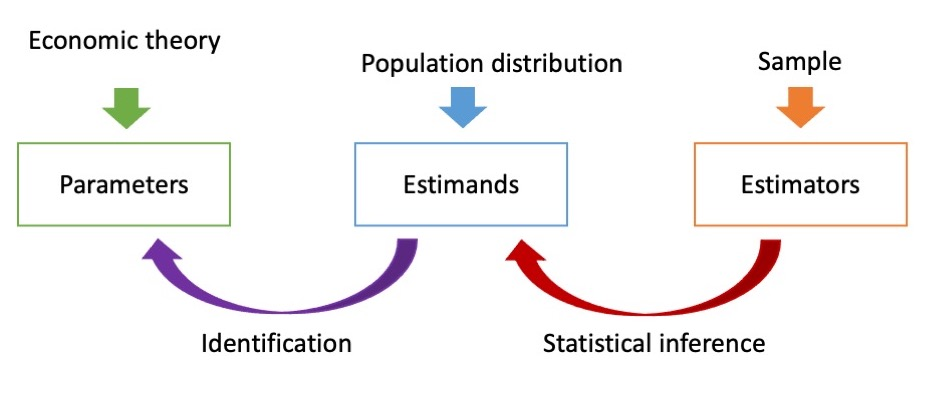
\includegraphics[width=0.9\linewidth]{BigPicture.jpg}
\end{center}
\vspace{-0.2cm}

\begin{itemize}
\item
\textbf{Statistics}: how does the sample data we observe relate to observable features of the population we're interested in? 
\smallskip

\item
\textbf{Identification}: how do observable features of population relate to target parameters of interest? 
\smallskip
\pause{}

\item
For both these tasks, we need a mathematical language for talking about how data is generated. Enter \textbf{probability and statistics}


\end{itemize}

\end{frame}

\begin{frame}
	\centering
	
\includegraphics[width = 0.5 \linewidth]{poppy_stick.jpg}
\end{frame}



\begin{frame}{Outline}
	
	1. Random Variables and Probability Distributions
	\vspace{0.8cm}
	
	2. Means and Variances
	\vspace{0.8cm}

	3. Identification in Experiments 
	\vspace{0.8cm}
		
	4. Random Sampling and Sample Means
	
	\vspace{0.8cm}
	5. Hypothesis Testing and Inference
	
\end{frame}


\begin{frame}{Random Variables}
\begin{wideitemize} 
\item
Probability theory formalizes the study of \textbf{random processes}\pause{}
\bigskip

\item What are some examples of a random process?\pause{}\smallskip
\begin{itemize}
	\item Flip a coin -- is it heads or tails? \smallskip
	\item Survey a random household in US -- what is their income? 
\end{itemize}
\pause{}
\bigskip

\item The realization of a random process is called a \textbf{random variable}.


\end{wideitemize}

\end{frame}

\begin{frame}{Some Terminology}

\begin{itemize}
\item \textbf{Outcomes} are mutually exclusive results of a random process (e.g. ``heads'' and ``tails'' are the outcomes of a single coin toss)
\vspace{0.1cm}\pause{}
\item The \textbf{probability} of an outcome captures its likelihood of occurring (i.e. frequency of its occurrence in repeated runs of the process)
\vspace{0.1cm}\pause{}
\item The \textbf{sample space} is the set of all possible outcomes
\vspace{0.1cm}\pause{}
\item An \textbf{event} is a subset of the sample space; its probability is the sum of probabilities of the included outcomes
\end{itemize}
\vspace{0.4cm}
\pause{}
Example: I toss two fair coins in the air\pause{}

\begin{itemize}
\item What are the possible outcomes (sample space)?
\vspace{0.1cm}\pause{}
\item What is the probability of seeing at least one head (an event)?
\end{itemize}

\end{frame}

\begin{frame}{Random Variables and CDFs}
\begin{wideitemize}
\item
A \textbf{random variable} is a numerical summary of a random process (formally, a real-valued function defined on the sample space)

\begin{itemize}
\item E.g. $X$ counts the number of heads we see 
\end{itemize}
\pause{}

\item A real-valued random variable is characterized by its \textbf{cumulative distribution function} (CDF), 

$$F(x) = Pr( X \leq x ) $$

\noindent which tells us the probabilty that $X$ is some value $x$ or below
\medskip\pause{}
\begin{itemize}
\item Note: we'll typically use lower-case letters like ``$x$'' to denote realizations (i.e. non-random numbers) of random variables like ``$X$'' ...
\end{itemize}

\end{wideitemize}
\end{frame} 

\begin{frame}
	\centering
	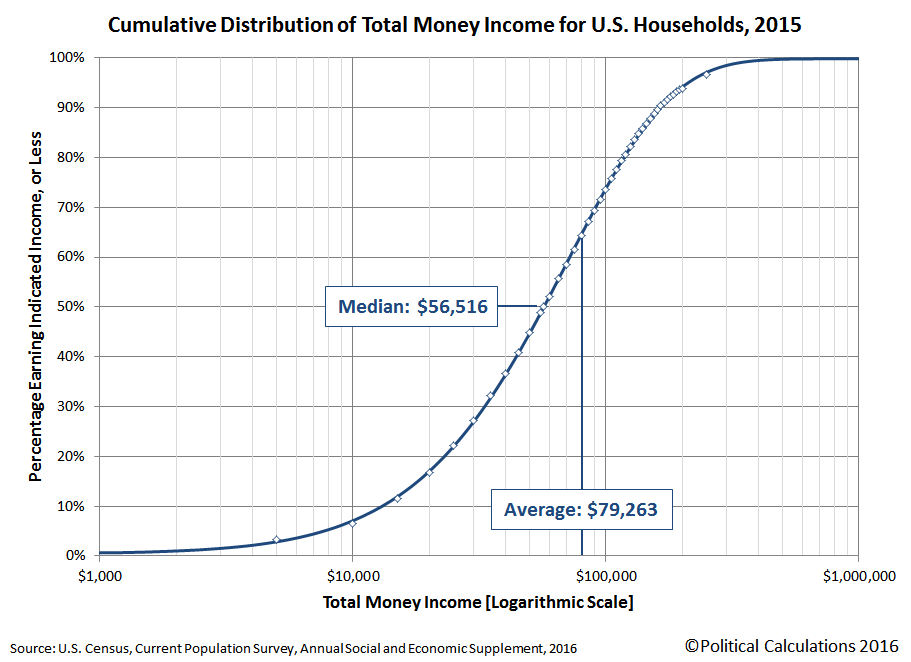
\includegraphics[width = 0.8\linewidth]{cdf-income}
	
	\begin{itemize}
		\item
		In 2016, around half of US households earned \$56K or less\smallskip
\pause{}
		\item Formally: $F(56,516)=0.5$
	\end{itemize}
\end{frame}



\begin{frame}{We All Need Some Support...}
	
\begin{wideitemize}
	\item
	The \textbf{support} of a random variable $X$, denoted $\mathbb{X}$, is the set of values that $X$ can take
	
		\begin{itemize}
			\item 
			If $X$ is months in the year you were employed, $\mathbb{X} = \{0,1,...,12\}$
			
			\item
			If $X$ is your income, then $\mathbb{X} = \mathbb{R}_{\geq 0}$ (approximately)
		\end{itemize}
	\smallskip\pause{}

	\item
	If the support of $X$ is finite (e.g. $\{0,1\}$), we say $X$ is \textbf{discrete}
	
	\item
	If the support of $X$ is a continuum (e.g. $\mathbb{R}$ or $[0,1]$), we say $X$ is \textbf{continuously distributed}  (technically, if the CDF is differentiable)
\end{wideitemize}

\end{frame}


\begin{frame}{Density and Mass Functions}

\begin{itemize}
	\item 
	If $X$ is discrete, we define the probability mass function (PMF) as the probability that $X$ takes on each value in the support: 
	\vspace{-0.2cm}
	$$p(x) = Pr(X =x )$$
	\pause
\vspace{-0.4cm}
	\begin{itemize}
	\item
	The CDF of a discrete random variable is then
	$$F(x) = \sum_{x' \leq x} p(x') $$ 
	\end{itemize}

	\pause
	\item
	For a continuous random variable, we define the probability density function (PDF) as $f(x) = \dfrac{d}{dx} F(x)$, implying a CDF of 
	$$F(x) = \int_{-\infty}^{x} f(t) dt$$
	
	\pause
	\item
	Notational note: both $p(x)$ and $f(x)$ are used for PDFs/PMFs
\end{itemize}

\end{frame}


\begin{frame}{}
\vspace{0.2cm}
Example of a discrete random variable: number of wifi connection failures 

\begin{itemize}
\item Here's the PMF; what is the CDF?
\end{itemize}

\begin{center}
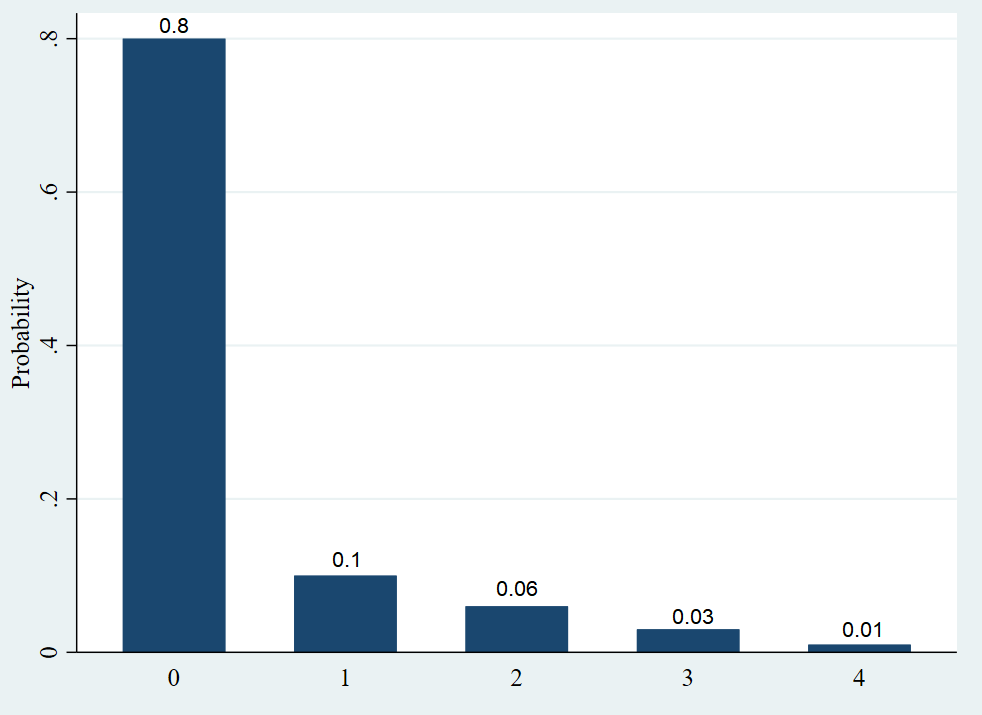
\includegraphics[scale=0.35]{simple_pmf.png}
\end{center}

\end{frame}

\begin{frame}{}
\vspace{0.2cm}
Example of a continuous random variable: commuting time

\begin{itemize}
\item Here's the PDF; what is the CDF?
\end{itemize}

\begin{center}
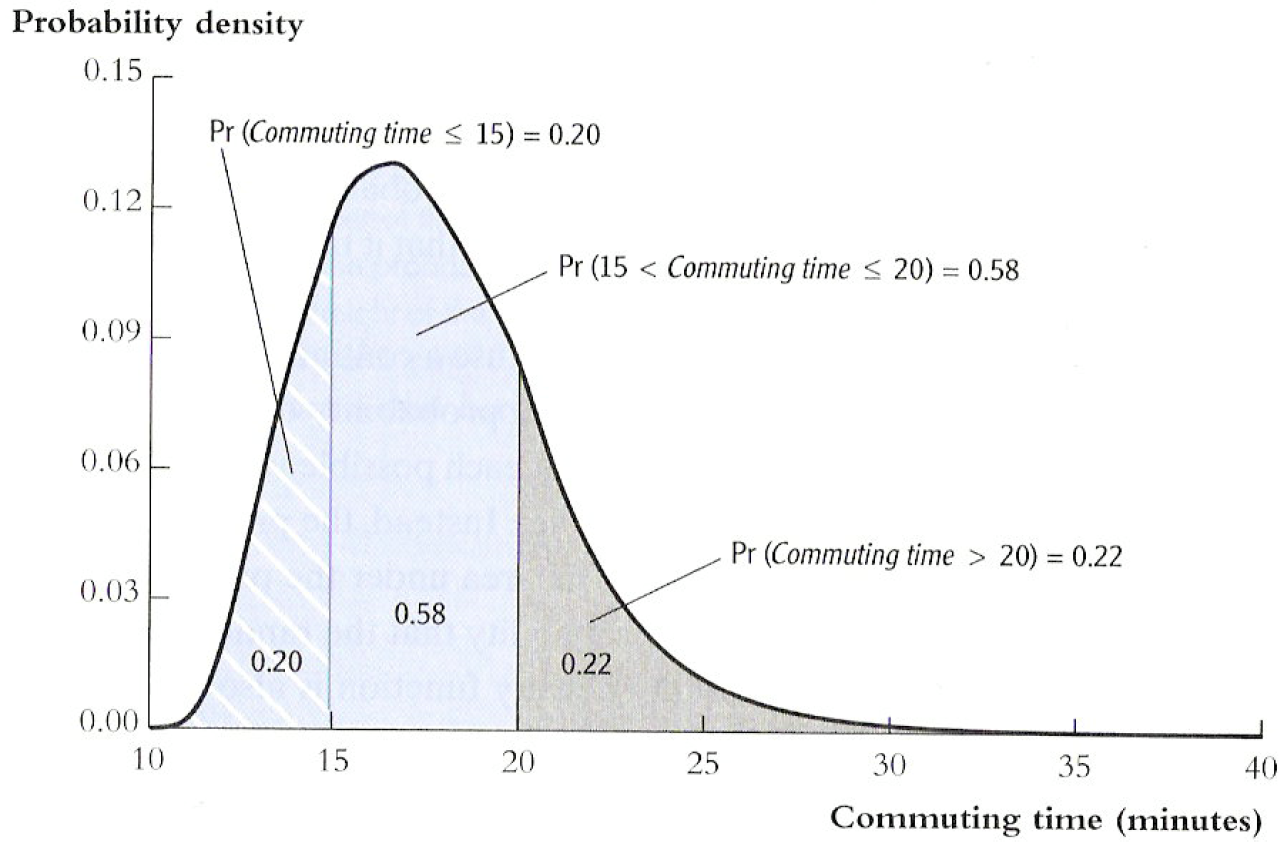
\includegraphics[scale=0.35]{simple_pdf.png}
\end{center}

\end{frame}

\begin{frame}{Properties of PDFs/CDFs}
\vspace{0.2cm}
\begin{itemize}
\item Key properties of CDFs $F(x)=Pr(X\le x)$: 
\smallskip

\begin{itemize}
\item Non-decreasing: $F(x)\ge F(x^\prime)$ if $x > x^\prime$
\vspace{0.1cm}
%\item Right-continuous: $\forall \varepsilon>0$, $\exists \delta>0$ s.t. $|P(x)-P(c)<\varepsilon|$, $\forall |x-c|<\delta$
%\vspace{0.1cm}
\item Satisfies $\lim_{x\rightarrow -\infty} F(x)=0$ and $\lim_{x\rightarrow +\infty}F(x)=1$
\end{itemize}
\vspace{0.5cm}
\pause{}

\item Corresponding properties of PDFs $f(x)=\frac{\partial}{\partial x}F(x)$: 
\smallskip

\begin{itemize}
\item Non-negative: $f(x)\ge 0$ for all $x\in\mathbb{X}$
\vspace{0.1cm}
\item Satisfies $\int_{x\in\mathbb{X}}f(x)dx=1$
\vspace{0.1cm}
\item For PMFs: $\sum_{x\in\mathbb{X}}p(x)=1$
\end{itemize}
\end{itemize}

\end{frame}


\begin{frame}{Bernoulli Distributions}
\vspace{0.1cm}
An important discrete distribution: Bernoulli $X\in\{0,1\}$\pause{}

\begin{itemize}
\item Examples: indicator for college completion, or whether a coin comes up "heads" (sometimes called a ``dummy variable'')
\vspace{0.1cm}\pause{}
\item PMF: 
\vspace{-0.4cm}
\begin{align*}
p(x)=
\begin{cases}
1-\pi, & x=0\\
\pi, & x=1
\end{cases}
\end{align*}
for some $\pi\in[0,1]$
\vspace{0.1cm}\pause
\item $\pi$ is the mean (expectation) of $X$, which we'll define formally soon
\vspace{0.1cm}\pause{}
\item Written $X\sim Bernoulli(\pi)$
\vspace{0.1cm}\pause{}
\item Note this is the \emph{only} distribution of any binary $X$
\end{itemize}

\end{frame}

\begin{frame}{Normal and Uniform Distributions}
\vspace{0.1cm}
An important continuous distribution: Normal $X\in\mathbb{R}$

\begin{itemize}
\item Example: the log of annual income (approximately)
\vspace{0.1cm}
\item PDF: $f(x)=\frac{1}{\sqrt{2\pi\sigma^2}}\exp\left(-\frac{1}{2}\frac{(x-\mu)^2}{\sigma^2}\right)$ for $x\in\mathbb{R}$ and $\sigma>0$
\vspace{0.1cm}
\item Here $\mu$ is the mean of $X$ and $\sigma^2$ is its variance (also defined soon)
\vspace{0.1cm}
\item Written $X\sim\mathrm{N}(\mu,\sigma^2)$
\vspace{0.1cm}
\item Useful property: if $X$ is normally distributed then so is $aX+b$ for any non-random $a$ and $b$ 


	\centering
\includegraphics<1>[width = 0.4 \linewidth]{normalpdf.jpeg}

\pause
\end{itemize}
\vspace{0.3cm}
Another continuous distribution worth knowing: Uniform $X\in (a,b)$
\pause{}

\begin{itemize}
\item Example: random lottery numbers (approximately)
\vspace{0.1cm}\pause{}
\item PDF: $f(x)=\frac{1}{b-a}$ for $x\in(a,b)$
\vspace{0.1cm}\pause{}
\item Written $X\sim\mathrm{U}(a,b)$; also closed under linear transformations
\end{itemize}

\end{frame}

\begin{frame}{Joint Distributions}
\vspace{0.2cm}
Many interesting economic questions involve features of the \textbf{joint distribution} of two or more random variables

\begin{wideitemize}
\item E.g. How do earnings ($Y$) and schooling levels ($X$) vary together?\pause{}

\item The CDF for the joint distribution is defined by
\vspace{-0.3cm}

$$F(x,y) = Pr(X \leq x, Y \leq y),$$
\noindent the probability that $X \leq x$ and $Y \leq y$.

\pause
\item For discrete ($X$,$Y$), we define joint PMF $p(x,y)=Pr(X=x,Y=y)$

\pause
\item For continuous ($X$,$Y$), we define joint PDF $f(x,y)=\frac{\partial^2}{\partial x \partial y}F(x,y)$
\end{wideitemize}
\vspace{0.5cm}
\pause{}

When dealing with multiple random variables, we sometimes refer to the distribution of an individual variable as its \textbf{marginal distribution}\pause{}

\begin{itemize}
\item Linked to the joint distribution by, e.g., $p(x)=\sum_{y\in\mathbb{Y}}p(x,y)$
\end{itemize}

\end{frame}

\begin{frame}{Conditional Distributions}

Combining joint and marginal distributions gives us the \textbf{conditional distribution} of one random variable given another

\begin{itemize}
\item Intuitively, the conditional distribution $Y|X=x$ is the distribution of $Y$ among the sub-population with $X=x$
	
\item Cond'l PMF $p(y\mid x)=Pr(Y=y\mid X=x)=\frac{Pr(Y=y,X=x)}{Pr(X=x)}=\frac{p(y,x)}{p(x)}$\pause{}
\item E.g. the distribution of earnings given college completion
\end{itemize}
\vspace{0.5cm}\pause{}

Leads immediately to \emph{Bayes' rule}:
\vspace{-0.4cm}
\begin{align*}
p(y\mid x)=p(x\mid y)\frac{p(y)}{p(x)}
\end{align*}

\end{frame}

\begin{frame}{Random Variables and Probability Distributions XI}
\vspace{0.2cm}
Conditional PDFs of annual income given college completion:

\begin{center}
\includegraphics[scale=0.6]{stata12.png} 

\includegraphics[scale=0.55]{stata13.png}
\end{center}

\end{frame}


\begin{frame}{Independence}

\begin{wideitemize} 
	
\item
An important concept in this course will be \textbf{independence}.

\item
Intuitively, independence says that knowing the value of $X$ tells us nothing about the value of $Y$


\item
Formally, $X,Y$ are independent ($X \indep Y$) if the conditional PDF/PMF of $Y|X=x$ is the same as the unconditional one: 	
$$ p(y\mid x)=p(y), \forall (y,x)$$


\pause
\item 
Example: if $D$ is a randomly assigned treatment, $D \indep (Y(1),Y(0))$. 
\pause
\begin{itemize}
	\item 
	Understanding check: does this imply that $D \indep Y$?
\end{itemize}

\pause 

\item
\textbf{Conditional independence} is defined similarly. $Y \indep X \mid W$ if 
$$ p(y\mid x,w)=p(y|w), \forall (y,x,w)$$

\item
Intuitively, $X$ tells us nothing about $Y$ once we know $W$.
\end{wideitemize}
\end{frame}

\begin{frame}{Multivariate Normals}

\vspace{0.2cm}
An important multivariate distribution: joint normal $\mathbf{X}\in\mathbb{R}^K$

\begin{itemize}
\item Parameterized by a (mean) vector $\boldsymbol{\mu}\in\mathbb{R}^K$ and a positive-definite (variance-covariance) matrix $\boldsymbol{\Sigma}\in\mathbb{R}^K\times\mathbb{R}^K$
\vspace{0.1cm}
\item Note: In general I will be using \textbf{boldface} to indicate vectors/matrices
\end{itemize}

\vspace{0.4cm}\pause{}

Many useful facts; here's a few. If $(X,Y)^\prime$ is joint-normally distributed:

\begin{itemize}
\item The marginal distributions of $X$ and $Y$ are normal
\vspace{0.1cm}
\item The conditional distributions of $X\mid Y$ and $Y\mid X$ are normal
\vspace{0.1cm}
\item Any fixed linear combination $aX+bY+c$ is normally distributed
\end{itemize}

\end{frame}


\begin{frame}{Bivariate Normal PDF}
\begin{center}
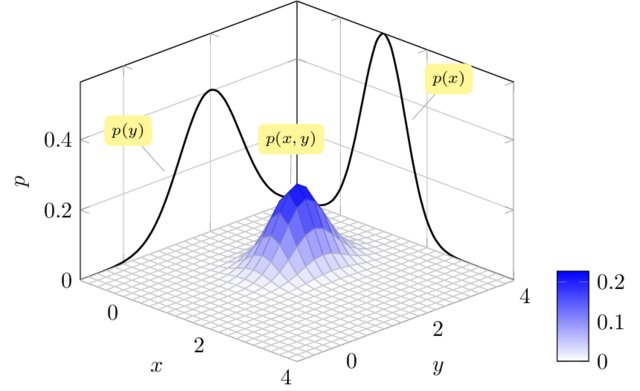
\includegraphics[scale=1.5]{binormal.jpg}
\end{center}
\end{frame}

\begin{frame}{Outline}
	
	\textcolor{red!75!green!50!blue!25!gray}{1. Random Variables and Probability Distributions}$\checkmark$
	\vspace{0.8cm}
	
	2. Means and Variances 
	\vspace{0.8cm}
	
	\textcolor{red!75!green!50!blue!25!gray}{3. Identification in Experiments}
	\vspace{0.8cm}
	
	\textcolor{red!75!green!50!blue!25!gray}{4. Random Sampling and Sample Means}
	
	\vspace{0.8cm}
	\textcolor{red!75!green!50!blue!25!gray}{5. Hypothesis Testing and Inference}
	
\end{frame}

\begin{frame}{Means}

\begin{wideitemize}

\item
We are often interested in the average of economic random variables (e.g. household income)

\item\pause{}
The \textbf{mean}/\textbf{expectation} of $X$ is its probability-weighted typical value


\begin{itemize}
\item For discrete random variables:
\vspace{-0.1cm}
\begin{align*}
E[X]=\sum_{x\in\mathbb{X}}p(x)x=x_1Pr(X=x_1)+\dots + x_KPr(X=x_K)
\end{align*}\pause{}
\vspace{-0.2cm}
Interpretation: long-run average of $X$ over repeated draws\pause{}

\vspace{0.5cm}
\item For continuous random variables, $E[X]=\int_{x\in\mathbb{X}}f(x)xdx$\pause \\ Caution: may not exist if $p(x)$ puts high probability on extreme $x$
\end{itemize}
\vspace{0.1cm}\pause

\item \textbf{Important fact:} The expectation operator is \emph{linear}: $E[a+bX]=a+bE[X]$ for  constants $(a,b)$
\vspace{0.1cm}

\begin{itemize}
\item Easily proved from the above definitions (make sure you can!)
\end{itemize}
\end{wideitemize}

\end{frame}



\begin{frame}{Calculating Means: a Simple Example}
	\begin{wideitemize}
		
		\item
		Let $X$ be the realization of a fair die. What is $E[X]$? 
		
		\smallskip
		\pause
		\item
		By definition,
		$$E[X] = Pr(X=1) \times 1 + Pr(X=2) \times 2 + .... + Pr(X=6) \times 6$$
		
		\pause
		\item
\smallskip
		If the die is fair, $Pr(X=1) =...=Pr(X=6) = \frac{1}{6}$
		
		\pause 
		\item 
		Plugging this in, we have
		
		$$E[X] = \frac{1}{6} (1+...+6) = 3.5$$
		
	\end{wideitemize}	
\end{frame}



\begin{frame}{Variances}
\vspace{0.2cm}
\textbf{Variances} measure the squared spread of a distribution: 

\begin{itemize}
\item $Var(X)=E\left[(X-E[X])^2\right]\pause{}=E\left[X^2\right]-E\left[X\right]^2$ (why?)
\vspace{0.1cm}\pause{}
\item The \emph{standard deviation} of $X$ is $Std(X)=\sqrt{Var(X)}$; it captures the ``typical'' deviation of $X$ from its mean
\end{itemize}
\vspace{0.2cm}
\pause{}

Variance of a linear transformation: 
\begin{align*}
Var(a+bX)=&\pause{}E[(a+bX-E[a+bX])^2]\pause{} \\
 = &E[(a+bX-a-bE[X])^2]\pause{} \\
= & b^2 E[(X-E[X])^2]\pause{} \\
 =& b^2Var(X)
\end{align*}

\pause{}
This implies that $Std(a + bX) = b \cdot Std(X)$.
	\begin{itemize}
		\item 
		Intuitively, if I measure income in cents, the standard deviation should be 100 times if I measure it in dollars
	\end{itemize}

\end{frame}


\begin{frame}{Covariances}
\vspace{0.2cm}
\emph{Covariance} measures the linear association between two variables: 

\begin{itemize}
\item $Cov(X,Y)=E\left[(X-E[X])(Y-E[Y])\right]=E[XY]-E[X]E[Y]$
\vspace{0.1cm}\pause{}
\item Notice how $Cov(X,X)=E\left[(X-E[X])^2\right]=Var(X)$
\vspace{0.1cm}\pause{}
\item The \emph{correlation} between $X$ and $Y$ is $Corr(X,Y)=\frac{Cov(X,Y)}{Std(X)Std(Y)}$
\end{itemize}
\vspace{0.3cm}
\pause{}

$Cov(X,Y)>0$ means $X$ tends to be above its mean when $Y$ is above its mean (and vice versa)\pause{}

\begin{itemize}
\item $Corr(X,Y)$ is a \emph{unit free} (standardized) measure of linear association
\vspace{0.1cm}\pause{}
\item If $X$ and $Y$ are independent, then $Cov(X,Y)=Corr(X,Y)=0$
\vspace{0.1cm}\pause{}
\item But \uline{not} vice-versa! Independence is a stronger notion of association 
\end{itemize}

\end{frame}

\begin{frame}{Examples of Correlations}

\begin{center}
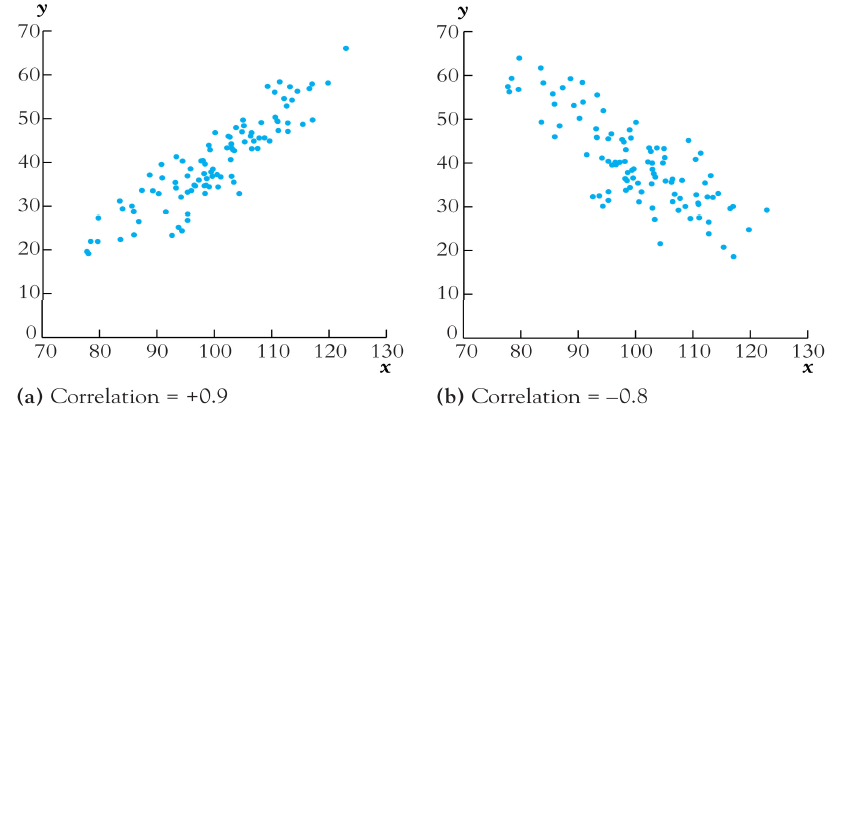
\includegraphics[scale=0.35]{corr2.png} 
\end{center}

\end{frame}

\begin{frame}{Examples of Correlations}

\begin{center}
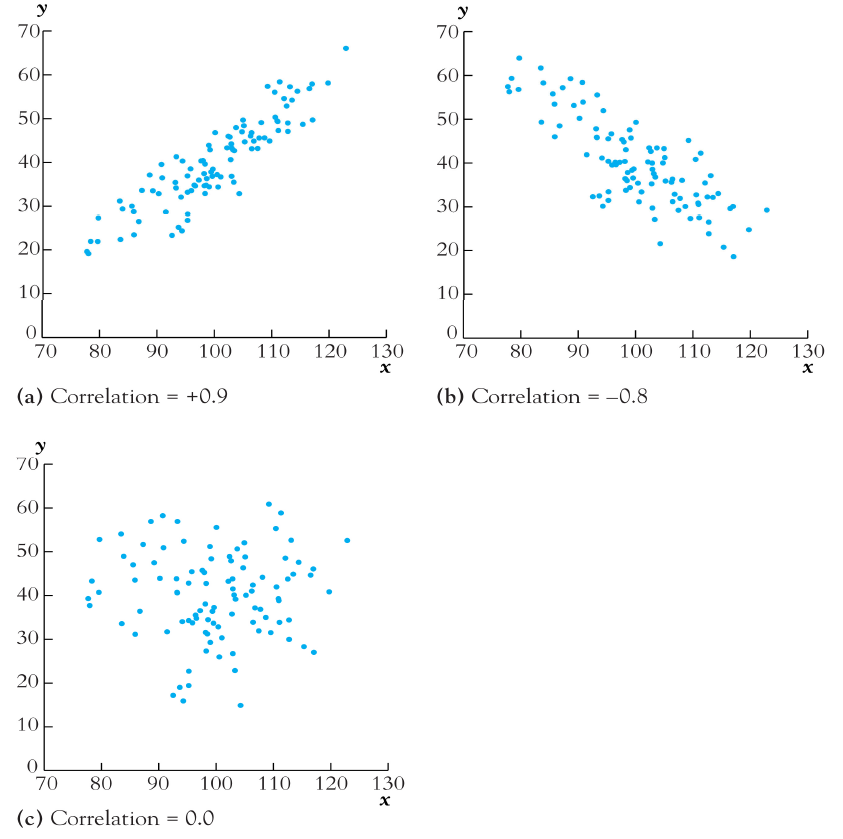
\includegraphics[scale=0.35]{corr3.png} 
\end{center}

\end{frame}

\begin{frame}{Examples of Correlations}

\begin{center}
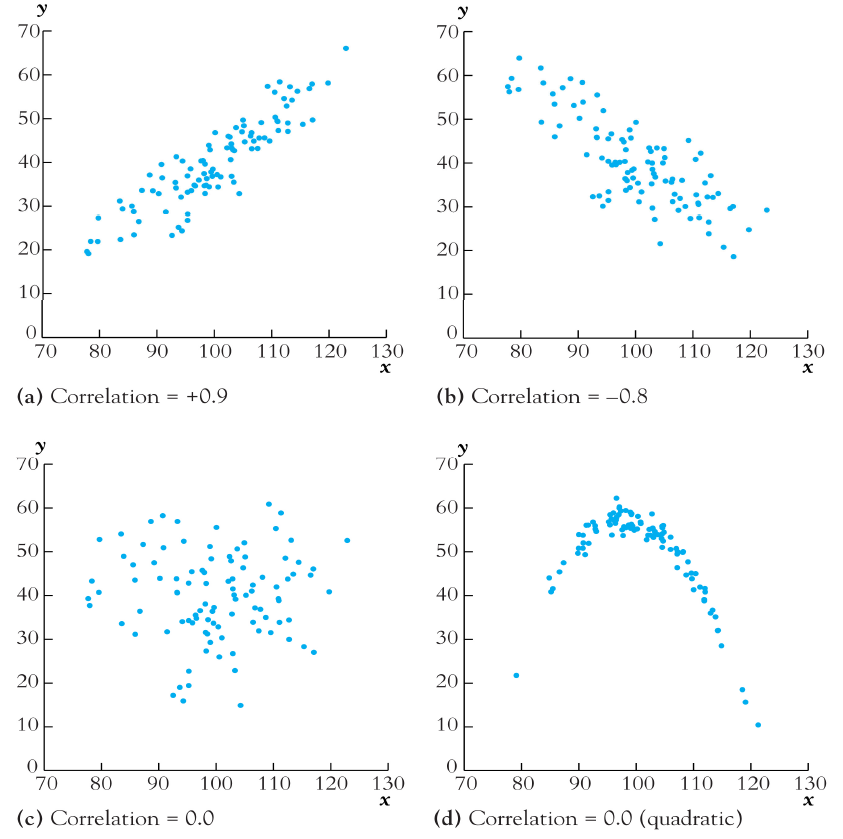
\includegraphics[scale=0.35]{corr4.png} 
\end{center}

\end{frame}

\begin{frame}{Means/Variances of Linear Combinations}
\begin{wideitemize}

\item
Expectations are linear: $E[aX+bY+c]=aE[X]+bE[Y]+c$ 

\pause

\item Variances are ``quadratic'':  $Var(aX+bY+c)=a^2Var(X)+2abCov(X,Y)+b^2Var(Y)$

\pause
\item
Covariances are linear: $Cov(aX+c,bY+d)=abCov(X,Y)$ \\ and $Cov(X+Z,Y)=Cov(X,Y)+Cov(Z,Y)$

\end{wideitemize}

\end{frame}

\begin{frame}{Conditional Expectations}
\vspace{0.2cm}
In economics we are especially interested in \textbf{conditional expectations}

\begin{itemize}
\item What is average of $Y$ when $X=x$ (e.g. what are the average earnings among people who went to Brown)?
\pause 
	
\item Conditional expectation function (CEF): \\$E[Y\mid X=x]=\sum_{y\in\mathbb{Y}} y p(y\mid x)$ if discrete \\
$E[Y\mid X=x]=\int_{y\in\mathbb{Y}} y f(y\mid x) dy$ if continuous

\vspace{0.1cm}\pause{}
\item We sometimes write $E[Y\mid X]$ for the \uline{random} CEF evaluated at $X$
\vspace{0.1cm}\pause{}
\item Say $Y$ is \emph{mean independent} of $X$ when $E[Y\mid X=x]=E[Y]$ for all $x$
\vspace{0.1cm}\pause{}
\item Conditioning on $X$ makes functions of it constant: e.g. $E[f(X)+g(X)Y|X=x]=f(x)+g(x)E[Y|X=x]$ for any $f(\cdot)$, $g(\cdot)$
\end{itemize}

\end{frame}


\begin{frame}{Conditional Expectation Example}
	\vspace{0.2cm}
	CEF of (log) annual income given years of schooling
	
	\begin{center}
		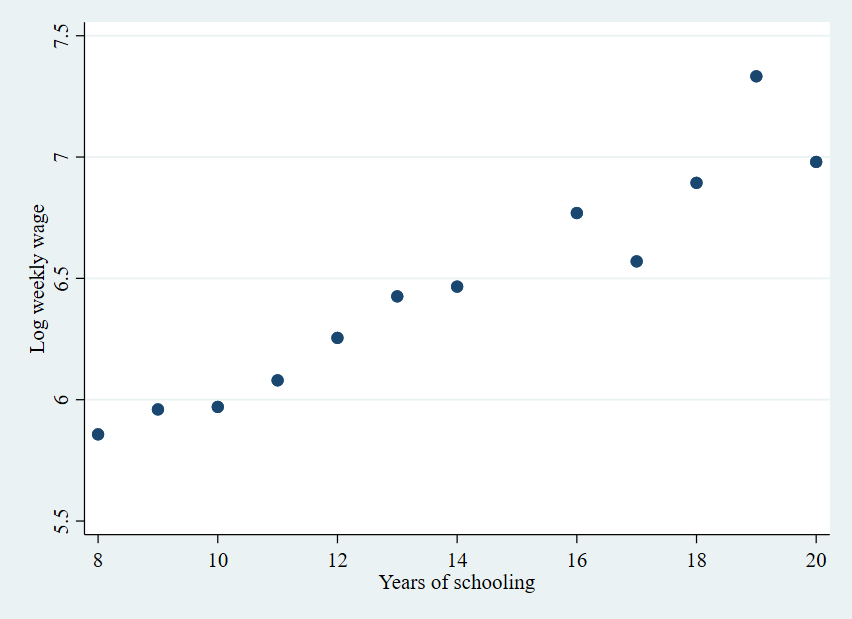
\includegraphics[scale=1.3]{stata2pre.png}
	\end{center}
	
\end{frame}

\begin{frame}{The Big LIE}
A very important result for us: the \textbf{Law of Iterated Expectations} (LIE)
\vspace{0.2cm}

Let's start with an example. Suppose I want to calculate the average height of people in the United States. The LIE says I can:  \vspace{0.2cm}

1) Compute the average height for men. \\ \vspace{0.2cm}

2) Compute the average height for women. \\ \vspace{0.2cm}

3) Average the average heights for men and women (proportional to the fraction who are women)

\vspace{0.2cm}
\pause
Mathematically, we have 

\begin{align*}
E[height] &= P(woman) E[height | woman] + P(man) E[height|man] \\ \pause{}
& =  E[ E[height | gender ]  ]	
\end{align*}
 



\end{frame}


\begin{frame}{The Big LIE}
	The formal version of the \textbf{Law of Iterated Expectations} (LIE) is:
	\begin{align*}
		E[Y]=E[E[Y\mid X]]\pause{}
	\end{align*}
	Note that the expectation on the LHS uses $p(y)$, while the outer expectation on the RHS uses $p(x)$ and the inner expectation uses $p(y\mid x)$
	
\end{frame}



\begin{frame}{Mean-Independence vs. Uncorrelatedness}
\vspace{0.2cm}
The LIE shows us that mean independence implies uncorrelatedness
\begin{align*}
Corr(X,Y)&\propto E[(X-E[X])(Y-E[Y])]\\ \pause{}
&=E[E[(X-E[X])(Y-E[Y])\mid X]]\\ \pause{}
&= E[(X-E[X])E[Y-E[Y]\mid X]]\\\pause{}
&= E[(X-E[X])(E[Y\mid X]-E[Y])]\\\pause{}
&= 0\text{, when $E[Y\mid X]=E[Y]$}
\end{align*}
\pause{}
\vspace{0.3cm}
Make sure you understand how we got each step! 
\vspace{0.5cm}
\pause{}

Converse does not hold: uncorrelated variables can be mean dependent
\pause{}

\begin{itemize}
\item Also, of course, independent $\implies$ mean independent (but not $\impliedby$)
\end{itemize}

\end{frame}


\begin{frame}{Quick Aside on Vector/Matrix Notation}

\vspace{0.2cm}
Often it will be useful to work with random vectors $\mathbf{X}=[X_1,\dots,X_N]^\prime$

\begin{itemize}
\item These will always be ``columns'' in this course, and denoted in bold
\vspace{0.1cm}
\item I will also use bold for matrices, with $K$ columns and $N$ rows
\end{itemize}\vspace{0.4cm}\pause{}

A useful reference for standard vector/matrix arithmetic/operators (e.g. transpose, inverse...) is \uline{The Matrix Cookbook }

\begin{itemize}
\item \url{www.math.uwaterloo.ca/~hwolkowi/matrixcookbook.pdf}
\end{itemize}\vspace{0.4cm}\pause{}

Expectations are elementwise: e.g. $E\left[\begin{bmatrix}X_{11}& X_{12}\\X_{21} & X_{22}\end{bmatrix}\right]=\begin{bmatrix}E[X_{11}]& E[X_{12}]\\E[X_{21}] & E[X_{22}]\end{bmatrix}$ 
\begin{itemize}
\item Define $Var\left(\begin{bmatrix}X_{1}\\X_{2}\end{bmatrix}\right)=\begin{bmatrix}Var(X_{1}) & Cov(X_{1},X_{2})\\Cov(X_{1},X_{2}) & Var(X_{2})\end{bmatrix}$ and $Cov\left(\begin{bmatrix}X_{1}\\X_{2}\end{bmatrix},\begin{bmatrix}Y_{1}\\Y_{2}\end{bmatrix}\right)=\begin{bmatrix}Cov(X_{1},Y_{1}) & Cov(X_{1},Y_{2})\\Cov(X_{2},Y_{1}) & Cov(X_{2},Y_{2})\end{bmatrix}$, etc
\end{itemize}

\end{frame}

\begin{frame}{Outline}
	
	\textcolor{red!75!green!50!blue!25!gray}{1. Random Variables and Probability Distributions}$\checkmark$
	\vspace{0.8cm}
	
	\textcolor{red!75!green!50!blue!25!gray}{2. Means and Variances} $\checkmark$
	\vspace{0.8cm}
	
	3. Identification in Experiments 
	\vspace{0.8cm}
	
	\textcolor{red!75!green!50!blue!25!gray}{4. Random Sampling and Sample Means}
	
	\vspace{0.8cm}
	\textcolor{red!75!green!50!blue!25!gray}{5. Hypothesis Testing and Inference}
	
\end{frame}

\begin{frame}{Identification in Experiments}
\begin{wideitemize}
\item
The theory we've covered so far is enough to show mathematically why experiments ``work'', at least from an identification perspective
\pause
\item Recall the \textit{potential outcomes} framework: 

\begin{itemize}
	\item
	$Y_i(1), Y_i(0)$ are outcomes of individual $i$ under treatment/control\smallskip
	
	\item
	Use these to model observed outcomes: $Y_i = D_i Y_i(1) + (1-D_i) Y_i(0)$ 
	
\end{itemize}

\pause
\item 
Suppose that we are interested in the average treatment effect:
$$ATE = E[Y_i(1) - Y_i(0) ]$$

\pause
\item
Suppose that for each person we assign $D_i$ by flipping a coin. This implies that $D_i \indep (Y_i(1),Y_i(0))$. Why?	
\end{wideitemize}		
\end{frame}

\begin{frame}{Using Randomization}
\vspace{0.2cm}
\begin{wideitemize}
\item
By virtue of the experiment, $D_i \indep (Y_i(1),Y_i(0))$.

\item
What is $\underbrace{E[Y_i | D_i = 1]}_{\text{Pop mean for treated units}}$?  	
\vspace{.3cm}
\pause
$$	E[Y_i|D_i=1] = E[Y_i(1) | D_i = 1] = E[Y_i(1)],$$
\noindent where the first equality uses the potential outcomes model and the second equality uses (mean) independence.

\pause
\item
Similarly, $E[Y_i | D_i = 0] =  E[Y_i(0) | D_i = 0] = E[Y_i(0)]$.

\pause
\item
Combining these results, we can see that
\vspace{-0.2cm}

$$\underbrace{E[Y_i | D_i = 1]}_{\text{Pop mean for treated}} - \underbrace{E[Y_i | D_i = 0]}_{\text{Pop mean for control}} = \underbrace{E[Y_i(1) - Y_i(0)]}_{\text{Avg treatment effect}} = \tau$$

Thus, the difference in treated/control population means in an experiment identifies the ATE!
\end{wideitemize}
\end{frame}


\begin{frame}{Identification under Conditional Unconfoundedness}
	\begin{wideitemize}
		\item
		Now suppose that $D_i \indep (Y_i(1), Y_i(0)) | \mathbf{X}_i$, where $\mathbf{X}_i$ is a vector of observable characteristic
		
		\item
		Called conditional unconfoundedness or \textbf{selection on observables}
		
		\pause
		\item
		Intuitively, conditional unconfoundedness says we effectively have an experiment among people with the same value of $\mathbf{X}_i$
\begin{itemize}
\item Implied by (unconditional) independence, but \emph{weaker}: allows non-randomness through $\mathbf{X}_i$
\end{itemize}
		
		\pause
		\item 
		Why might we believe conditional unconfoundedness? 
		\begin{itemize}
			\item 
			Stratified experiment: we randomize among people with same value of $\mathbf{X}_i$ (e.g., we hold a lottery for each state)
			
			\medskip
			\pause
			\item
			``Quasi-experiment''/``natural experiment'': we think $D_i$ is (effectively) as good as random among people with same value of $\mathbf{X}_i$
		\end{itemize}
	\end{wideitemize}
\end{frame}


\begin{frame}{Example -- Hot Days and Test Scores}
	
\begin{wideitemize}
\item
\href{https://www.nature.com/articles/s41562-020-00959-9}{\uline{Park et al (2021)}} study the impact of hot days ($D_i$) during the school year on test scores ($Y_i$)\smallskip
\begin{itemize}
	\item 
	Note Their $D_i$ is not binary, although we could imagine a binarized treatment, e.g. $D_i = 1[Hot days > 10]$
\end{itemize}

\item
Why do we think $D_i \not\indep (Y_i(1),Y_i(0))$? 
\pause
	\begin{itemize}
		\item 
		People in places with different climates may be different on other things
	\end{itemize}

\pause
\item
Park et al argue that $D_i \indep (Y_i(1),Y_i(0)) | X_i$, where $X_i$ is a measure of historical weather in $i$'s location 

	\begin{itemize}
		\item 
		Heat in a given year is effectively random conditional on historical weather patterns. 
	\end{itemize}

\item\pause{}
Does this seem reasonable to you? 

\end{wideitemize}	
	
\end{frame}


\begin{frame}{Park et al. (2021) Abstract}
	\centering
	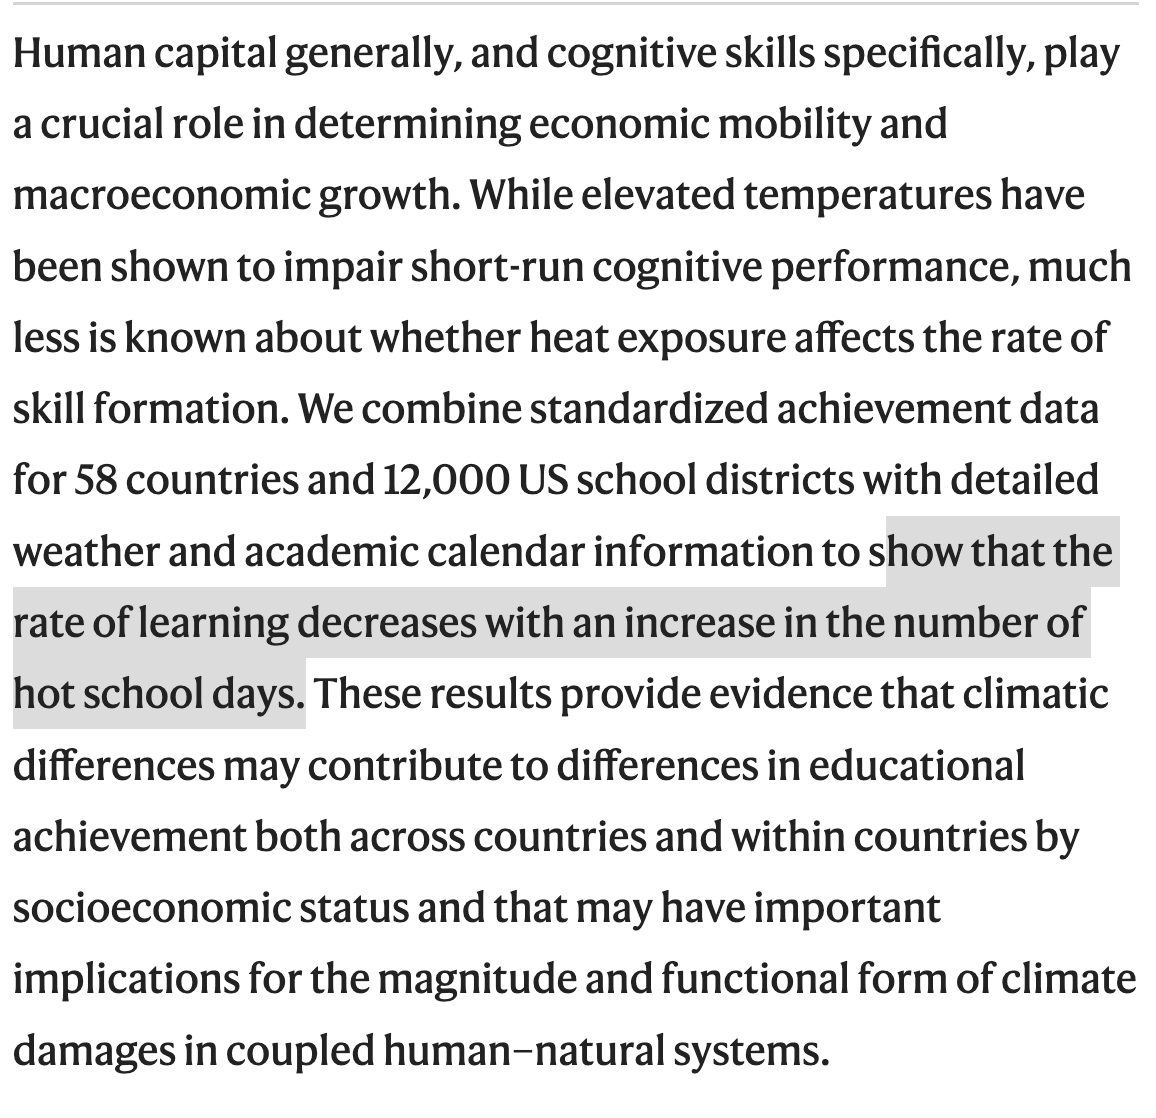
\includegraphics[width =0.6\linewidth]{park-heat}
\end{frame}

\begin{frame}{Example -- Returns to College Selectivity}
\begin{wideitemize}
\item
\href{https://academic.oup.com/qje/article-abstract/117/4/1491/1876022}{\uline{Dale and Krueger (2002)}} studied a Q similar to our ongoing example: \\
What is the effect on earnings of attending a selective college?

\item 
Clearly, $D_i \not\indep (Y_i(1),Y_i(0))$ because students who attend selective college will tend to have different academic ability. 

\pause
\item
Dale and Krueger argue that $D_i \indep (Y_i(1),Y_i(0)) | \mathbf{X}_i$, where $\mathbf{X}_i$ is the set of colleges to which someone applied and got admitted. 

\item
Essentially, they argue that once we know what colleges you applied/ were admitted to, where you choose to go is effectively random

\pause
\item
Do you believe this? Why might this assumption go wrong? 
\pause
	\begin{itemize}
		\item 
		Students who choose to go to selective college may still differ in family background, motivation, career plans, etc. 
	\end{itemize}
\end{wideitemize}
\end{frame}

\begin{frame}{Dale and Krueger (2002)}
	\centering
	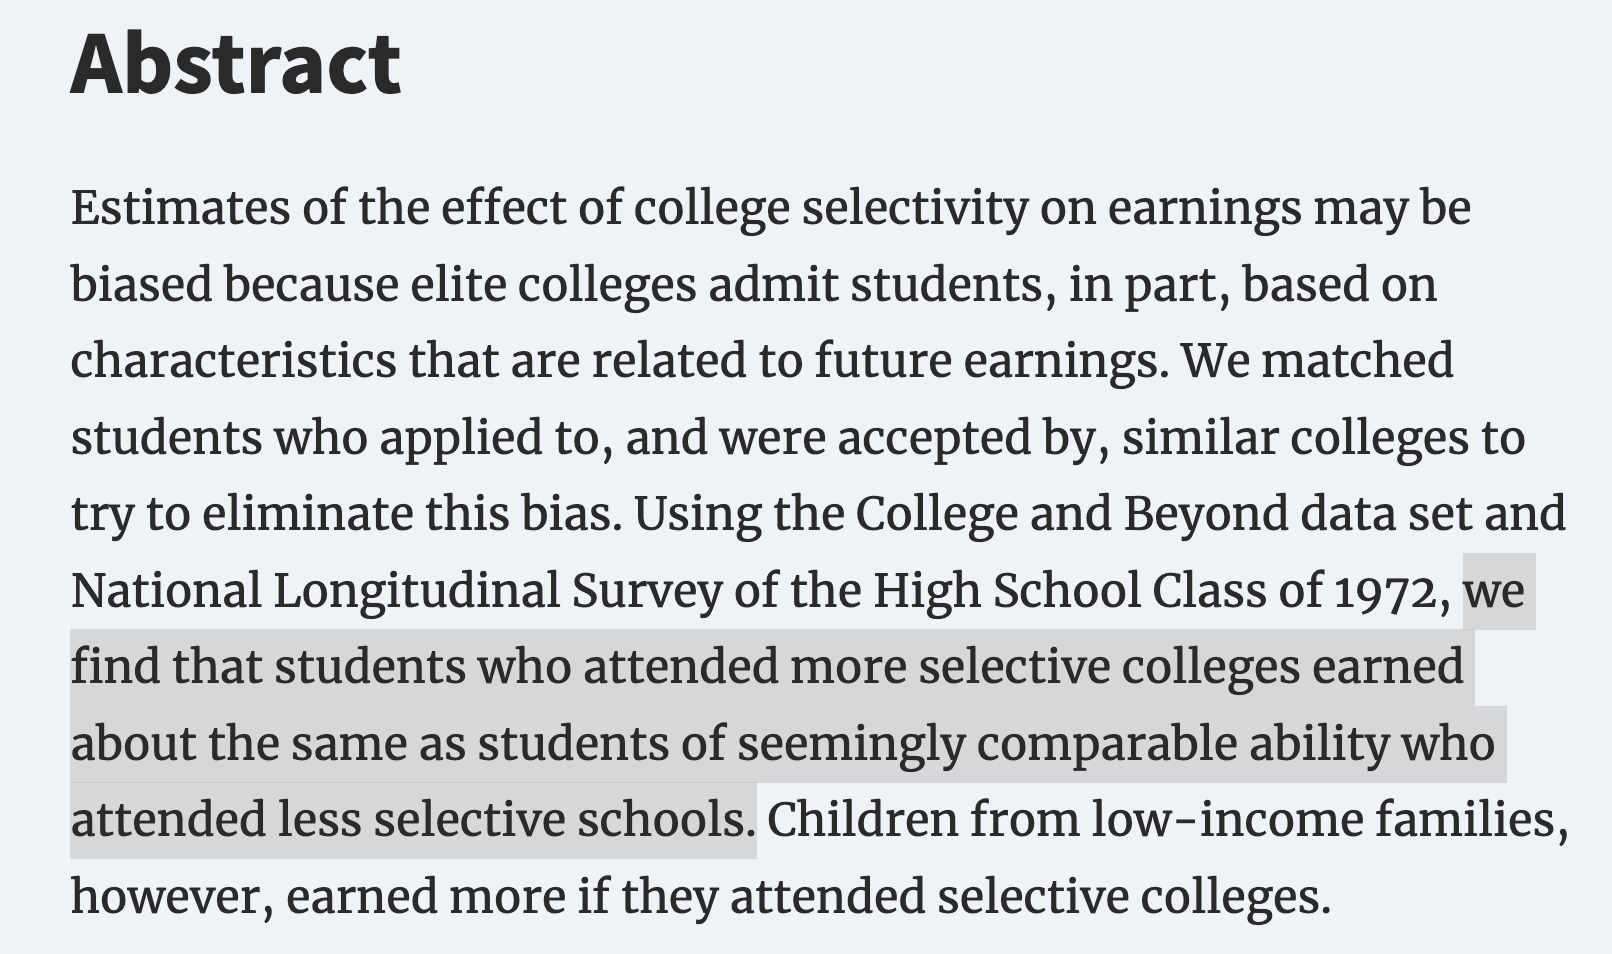
\includegraphics[width = 0.9\linewidth]{dale-krueger}
\end{frame}


\begin{frame}{Using Conditional Unconfoundedness}
\vspace{0.2cm}
	\begin{wideitemize}
		\item
		Suppose that $D_i \indep (Y_i(1), Y_i(0)) | \mathbf{X}_i$, where $\mathbf{X}_i$ is a vector of observable characteristics. 
		
		\item
		Similar to in the experiment, we have for all $\mathbf{x}$:
		$$E[Y_i | D_i = 1,\mathbf{X}_i= \mathbf{x}] = E[Y_i(1) | \mathbf{X}_i=\mathbf{x}].$$
		
		and 
		
		$$E[Y_i | D_i = 0,\mathbf{X}_i = \mathbf{x}] = E[Y_i(0) | \mathbf{X}_i =\mathbf{x}].$$
		
		\pause
		\item
		This implies that
		$$\small \underbrace{E[Y_i | D_i = 1, \mathbf{X}_i= \mathbf{x}] }_{\text{Pop avg treated w/ $\mathbf{X}_i= \mathbf{x}$}}- \underbrace{E[Y_i | D_i = 0, \mathbf{X}_i= \mathbf{x}]}_{\text{Pop avg control w/ $\mathbf{X}_i= \mathbf{x}$}} = \underbrace{E[Y_i(1) - Y_i(0) | \mathbf{X}_i= \mathbf{x}]}_{\text{ATE with $\mathbf{X}_i= \mathbf{x}$}} $$ 
		
		\pause
		\item 
		$E[Y_i(1) - Y_i(0) | \mathbf{X}_i= \mathbf{x}]$ is often called the \textit{conditional average treatment effect}, written $CATE(\mathbf{x})$. 	
	\end{wideitemize}	
\end{frame}



\begin{frame}{Using Conditional Unconfoundedness (cont.)}
\vspace{0.2cm}
	\begin{wideitemize}
		\item 
		We showed that under conditional unconfoundedness, $CATE(\mathbf{x}) = E[Y_i(1) - Y_i(0) | \mathbf{X}_i= \mathbf{x}] $ is identified.
		
		\item 
		Is the unconditional $ATE=E[Y_i(1) - Y_i(0)]$ also identified? 
		
		\pause
		\item
		Yes! Using the law of iterated expectations,
		$$E[ \underbrace{E[Y_i(1) - Y_i(0) | \mathbf{X}_i] }_{ CATE(\mathbf{X}_i) }  ] = E[Y_i(1) - Y_i(0)]$$
		
		\pause
		
		\item
		\textbf{Technical note}: Here we assume $E[Y_i | D_i = 1, \mathbf{X}_i= \mathbf{x}]$ and $E[Y_i | D_i =0,\mathbf{X}_i= \mathbf{x}]$ exist for every $\mathbf{x}$
		
		\pause
		\item
		Requires $0< Pr(D_i = 1 |\mathbf{X}_i= \mathbf{x}]) < 1$: called an \textbf{overlap} condition
		
		\item
		Intuitively, we need there to be some treated and some control units for each value of $X_i$, in order to learn about the \uline{overall} $ATE$
	\end{wideitemize}
\end{frame}


\begin{frame}{Learning about Population Means}
	
	\begin{wideitemize}
		\item We just showed that, in an experiment, the average treatment effect is identified as the difference in population means:
		
		$$E[Y_i | D_i = 1] - E[Y_i |D_i =0] = E[Y_i(1)-Y_i(0)]$$

		\item
		Similarly, under conditional unconfoundedness, the CATE is identified by a difference in conditional population means
		
		\pause
		\item
		But in practice, we don't see data for the whole population, so we don't know $E[Y_i | D_i = 1]$, $E[Y_i | D_i = 0]$, etc. 
		
		\pause
		\item
		We need to learn about these \textbf{estimands} from the observed sample 
		
		\item
		Enter \textbf{statistical inference...}
	\end{wideitemize}
	
\end{frame}



\begin{frame}{Outline}
	
	\textcolor{red!75!green!50!blue!25!gray}{1. Random Variables and Probability Distributions} $\checkmark$
	\vspace{0.8cm}
	
	\textcolor{red!75!green!50!blue!25!gray}{2. Means and Variances} $\checkmark$
	\vspace{0.8cm}
	
	\textcolor{red!75!green!50!blue!25!gray}{3. Identification in Experiments}  $\checkmark$
	\vspace{0.8cm}
	
	4. Random Sampling and Sample Means
	
	\vspace{0.8cm}
	\textcolor{red!75!green!50!blue!25!gray}{5. Hypothesis Testing and Inference}
	
\end{frame}



\begin{frame}{Defining a Sample}
	\begin{wideitemize}	
	
	\item
	To formalize the task of statistical inference, we need to specify how our observed data is drawn from the population
	
	\pause{}
	

	\item Baseline case: we observe an \emph{independent and identically distributed} (\emph{iid}) and  \textit{representative }sample of size $N$: e.g. $\mathbf{Y}=[Y_{1},Y_{2},\dots,Y_{N}]^\prime$
	
	\pause{}\smallskip
\begin{itemize}
	\item \emph{Independent}: $Y_i$ is independent of $Y_j$ for all $i\neq j$
	
\smallskip
	\pause{}
	\item \emph{Identically distributed}: $Y_i$ and $Y_j$ have the same distribution for all $i,j$

\pause{}
\smallskip
	\item
	\emph{Representative:} The distribution of $Y_i$ is the same as the distribution from the population we care about
	
\end{itemize}		
	\pause	
	\item	
	\emph{iid} and representative data is a useful baseline that's relatively easy to analyze, but it's important to realize it might not hold in practice
		\begin{itemize}
			\pause
\smallskip
			\item
			If we sample people in the same household together, not independent! 
		
\smallskip	
			\pause
			\item
			If we stratify sampling by state, not identical 
			\pause

\smallskip
			\item 
			In the Dewey v. Truman example, not representative! 
		\end{itemize}
	\end{wideitemize}

\end{frame}



\begin{frame}{The Mean and Variance of a Sample Average}
\vspace{0.2cm}
Suppose we are interested in learning the population mean $\mu=E[Y_i]$ from an \emph{iid} representative sample $\mathbf{Y}$ of size $N$\pause{} 
\pause{}
\begin{itemize}
\item A natural estimator is the \emph{sample mean}: $\hat{\mu}=\frac{1}{N}\sum_i Y_{i}$
\vspace{0.1cm}\pause{}
\item $\hat{\mu}$ is a function of the random data $\mathbf{Y}$. It is thus a random variable, and it has a distribution (sometimes called a ``sampling distribution'')
\end{itemize}
\vspace{0.4cm}
\pause{}

We can use what we've learned to derive the mean and variance of $\hat{\mu}$
\begin{align*}
E[\hat{\mu}]&=E\left[\frac{1}{N}\sum_i Y_i\right]=\pause\frac{1}{N}\sum_i E[Y_i]=\pause\mu\\\pause{}
Var(\hat{\mu})&=Var\left(\frac{1}{N}\sum_i Y_i\right)=\pause{}\frac{1}{N^2}\sum_iVar(Y_i)=\pause{}\sigma^2/N,
\end{align*}
where $\sigma^2=Var(Y_i)$ 
\pause{}

\begin{itemize}
\item Equation (1) says that $\hat{\mu}$ is \emph{unbiased}: its average value is $\mu$
\vspace{0.1cm}
\pause{}
\item Equation (2) says that the standard deviation of $\hat{\mu}$ from its mean (i.e. $\mu$) shrinks with the sample size $N$ ($\approx$ \emph{consistency})
\end{itemize}

\end{frame}

\begin{frame}{Random Sampling and Sample Means}
\vspace{0.2cm}
Simulating unbiasedness and consistency for estimating mean income:

\begin{center}
\includegraphics[scale=0.45]{stata18.png} \includegraphics[scale=0.5]{stata19.png}
\end{center}

\end{frame}

\begin{frame}{Simulations of Random Sampling}
\vspace{0.2cm}
Simulating unbiasedness and consistency for estimating mean income:

\begin{center}
\includegraphics[scale=0.45]{stata18.png} \includegraphics[scale=0.5]{stata20.png}
\end{center}

\end{frame}

\begin{frame}{Random Sampling and Sample Means}
\vspace{0.2cm}
Simulating unbiasedness and consistency for estimating mean income:

\begin{center}
\includegraphics[scale=0.45]{stata18.png} \includegraphics[scale=0.5]{stata21.png}
\end{center}

\end{frame}

\begin{frame}{Random Sampling and Sample Means}
\vspace{0.2cm}
Simulating unbiasedness and consistency for estimating mean income:

\begin{center}
\includegraphics[scale=0.45]{stata18.png} \includegraphics[scale=0.5]{stata22.png}
\end{center}

\end{frame}

\begin{frame}{Random Sampling and Sample Means}
\vspace{0.2cm}
Simulating unbiasedness and consistency for estimating mean income:

\begin{center}
\includegraphics[scale=0.45]{stata18b.png} \includegraphics[scale=0.5]{stata23.png}
\end{center}

\end{frame}

\begin{frame}{Random Sampling and Sample Means}
\vspace{0.2cm}
So: two reasons why $\hat{\mu}=\frac{1}{N}\sum_i Y_i$ is a good estimator of $\mu=E[Y_i]$:

\begin{itemize}
\item It is unbiased: $E[\hat{\mu}]=\mu$
\vspace{0.1cm}
\item Its variance shrinks to zero as the sample grows: $\lim_{N\rightarrow\infty}Var(\hat{\mu})=0$ 
\end{itemize}
\vspace{0.5cm}
\pause{}


In the next chapter we'll see another nice property of $\hat{\mu}$: when $N$ is large, its \emph{distribution} is approximately normal

\end{frame}

\begin{frame}{Random Sampling and Sample Means}
\vspace{0.2cm}
Given our interest in conditional means $\mu(x)=E[Y_i\mid X_i=x]$, we might also consider conditional sample averages of $Y_i$ given $X_i=x$
\pause{}


\begin{itemize}
\item This is easiest when $X_i$ is discrete with a small number of values $x$
\vspace{0.1cm}\pause{}
\item Natural estimator $\hat{\mu}(x)=\frac{1}{N_x}\sum_{i:X_i=x}Y_i$, where $N_x=|i:X_i=x|$ counts the number of observations with $X_i=x$
\end{itemize}
\vspace{0.4cm}
\pause{}

Following the same derivations as before, we have 
\begin{align*}
E[\hat{\mu}(x)]&=E[Y_i\mid X_i=x]=\mu(x)\\
Var(\hat{\mu}(x))&=Var(Y_i\mid X_i=x)/N_x
\end{align*}
\pause{}
\vspace{-0.2cm}

So this is an \emph{unbiased} estimator which is close to the truth as $N_x\rightarrow\infty$
\pause{}

\begin{itemize}
\item What if $X_i$ is not discrete, or $N_x\not\rightarrow\infty$? Coming soon...
\end{itemize}

\end{frame}

%\begin{frame}{Random Sampling and Sample Means V}
%\vspace{0.2cm}
%\uline{Fun with Notation}: we can write this CEF estimator as 
%\begin{align*}
%\hat{\mu}(x)=\frac{1}{N_x}\sum_{i:X_i=x}Y_i=\frac{\sum_{i}D_{ix}Y_i}{\sum_{i}D_{ix}}
%\end{align*}
%where $D_{ix}=\mathbf{1}[X_i=x]$ is an indicator for $X_i$ taking on value $x$ (why?)
%\vspace{0.4cm}
%\pause{}
%
%In vector form, we can write this as
%\begin{align*}
%\hat{\mu}(x)=(\mathbf{D_x}^\prime \mathbf{D_x})^{-1} \mathbf{D_{x}}^\prime \mathbf{Y}
%\end{align*}
%for $\mathbf{D_x}=[D_{x1},\dots,D_{xN}]^\prime$
%
%\pause{}
%\vspace{0.4cm}
%
%Furthermore if we collect $\mathbf{D}=[\mathbf{D_{x_1}},\mathbf{D_{x_2}},\dots,\mathbf{D_{x_K}}]$, then we can write the vector of CEF estimates $\hat{\boldsymbol\mu}=[\hat{\mu}(x_1),\hat{\mu}(x_2),\dots,\hat{\mu}(x_K)]^\prime$ as 
%\begin{align*}
%\hat{\boldsymbol\mu}=(\mathbf{D}^\prime \mathbf{D})^{-1} \mathbf{D}^\prime \mathbf{Y}
%\end{align*}\pause{}
%\vspace{-0.5cm}
%
%\begin{itemize}
%\item This shows $\hat{\boldsymbol\mu}$ is an ordinary least squares (OLS) linear regression estimator, which you'll learn to love soon...
%\end{itemize}
%
%\end{frame}

\begin{frame}{Outline}
	
	\textcolor{red!75!green!50!blue!25!gray}{1. Random Variables and Probability Distributions} $\checkmark$
	\vspace{0.8cm}
	
	\textcolor{red!75!green!50!blue!25!gray}{2. Means and Variances} $\checkmark$
	\vspace{0.8cm}
	
	\textcolor{red!75!green!50!blue!25!gray}{3. Identification in Experiments} $\checkmark$
	\vspace{0.8cm}
	
	\textcolor{red!75!green!50!blue!25!gray}{4. Random Sampling and Sample Means} $\checkmark$
	
	\vspace{0.8cm}
	5. Hypothesis Testing and Inference 
	
\end{frame}


\begin{frame}{Hypothesis Testing -- an Introduction}
\begin{wideitemize}

\item
We've shown that when $N$ gets large, the sample mean $\hat\mu$ gets close to the population mean $\mu$

\item
But what does ``close'' mean? 

\item
If the sample mean of income in our data is \$50,000, is it reasonable to think the population mean could be \$55,000? What about \$70,000? 

\pause
\item
\textbf{Hypothesis testing} helps us formalize the notion of ``close.''

\pause
\item
It tells us whether it is likely to see a sample mean of \$50,000 if the truth is \$55,000,  \$70,000, etc.

\end{wideitemize}
\end{frame}


\begin{frame}{Overview of Hypothesis Testing}

\begin{enumerate}
	\item 
	Specify a \textbf{null hypothesis} that the population mean is a particular value, $H_0: \mu = \mu_0$.
\smallskip
		\begin{itemize}
			\item 
			E.g. A population mean is \$55,000 would be $H_0: \mu = 55,000$
			\end{itemize}
	
	\medskip
	\pause
	\item
	Calculate how likely it would be to observe $\hat\mu$ at least this far from $\mu_0$ if the null is true. This is called a \textbf{$\mathbf{p}$-value}
	\medskip
	\pause
	\item
	\textbf{Reject} if the $p$-value is small, i.e.: it's unlikely that we would observe a $\hat\mu$ so far from $\mu_0$ if the null is true 
\smallskip
		\begin{itemize}
		\pause 
		\item
		A common threshold is $\alpha=0.05$ 
	\end{itemize}
	
	\vspace{.1cm}
	\pause
	\item
	
	Form a \textbf{confidence interval} that collects all the possible values of $\mu_0$ that we can't reject in this way
		\begin{itemize}
			\pause
			\item
			The CI, by construction, contains the true value $\mu$ in 95\% of the realizations of the data when $\alpha = 0.05$ 
		\end{itemize}
\end{enumerate}
	
\end{frame}


\begin{frame}{Hypothesis Testing with Normally Distributed $\hat\mu$}
\begin{itemize}
	\item 
	Let's work through all the steps in the special case: $\hat\mu \sim \mathrm{N}(\mu, \sigma^2/N)$ with $\sigma^2$ known. 
	\medskip
	\pause
	\item
	Why consider this case?
\smallskip
		\begin{itemize}
			\item 
			$\mathrm{N}(\mu, \sigma^2/N)$ is the exact distribution of $\hat\mu$ if $Y_i \overset{iid}{\sim} \mathrm{N}(\mu,\sigma^2)$ \pause
			\smallskip
			\item
			We'll show in the next chapter that even if $Y_i$ is not normal, $\hat\mu$ is approximately normal for large $N$
\smallskip\pause{}
\item We'll also show that with large $N$ we can estimate $\sigma^2$ arbitrarily well
		\end{itemize}

	\pause
	\item
	Suppose we wish to test the null hypothesis $H_0:\mu=\mu_0$ (e.g. average income is \$55,000)
	
	
	\item
	Let $\hat{t} = \dfrac{\hat\mu - \mu_0 }{ \sigma /\sqrt{N} }$, and note under the null hypothesis $\hat{t} \sim \mathrm{N}(0,1)$ 
	\begin{itemize}
	\pause
	\item
	The distribution of $\hat{t}$ is over repeated draws of the sample $(Y_1,...,Y_N)$.
		\end{itemize}
\end{itemize}
\end{frame}

\begin{frame}{Hypothesis Testing with Normally Distributed $\hat\mu$ (cont.)}
\begin{wideitemize}
\item
We've shown that under the null, $H_0:\mu=\mu_0$, $\hat{t} \sim \mathrm{N}(0,1)$.

\pause
\item What is $Pr( |\hat{t}| > t )$ for some $t \geq 0$? \pause
$$ Pr( |\hat{t}| > t ) = 1 - Pr(|\hat{t}| \leq t) \pause = 1 - Pr(  -t \leq \hat{t} \leq t  ) = \pause 1 - (\Phi(t) - \Phi(-t))$$ 
\vspace{-0.8cm}
\item
We define the $p$-value for the null $H_0: \mu = \mu_0$ as 
\begin{align*}
 p(\hat{t}) = 1 - (\Phi( |\hat{t} | ) - \Phi(- |\hat{t} |  )  ) \pause{} &= 1-  \left(  \Phi \left(  \frac{|\hat\mu - \mu_0|}{\sigma / \sqrt{N}} \right)  -  \Phi \left(  \frac{-|\hat\mu - \mu_0|}{\sigma / \sqrt{N}} \right) \right) 	\\
 &\pause{}= 2\left(1 -  \Phi \left(  \frac{|\hat\mu - \mu_0|}{\sigma / \sqrt{N}} \right)  \right) 
\end{align*}

 
\item
Intuitively, $p$ is the probability we would see a $|\hat{t}|$ at least this big if the null is true.

\end{wideitemize}	
\end{frame}

\begin{frame}{Illustration of P-Value Construction}
	
	
	\begin{center}
		Standard Normal PDF (mean zero, unit std. dev.)
		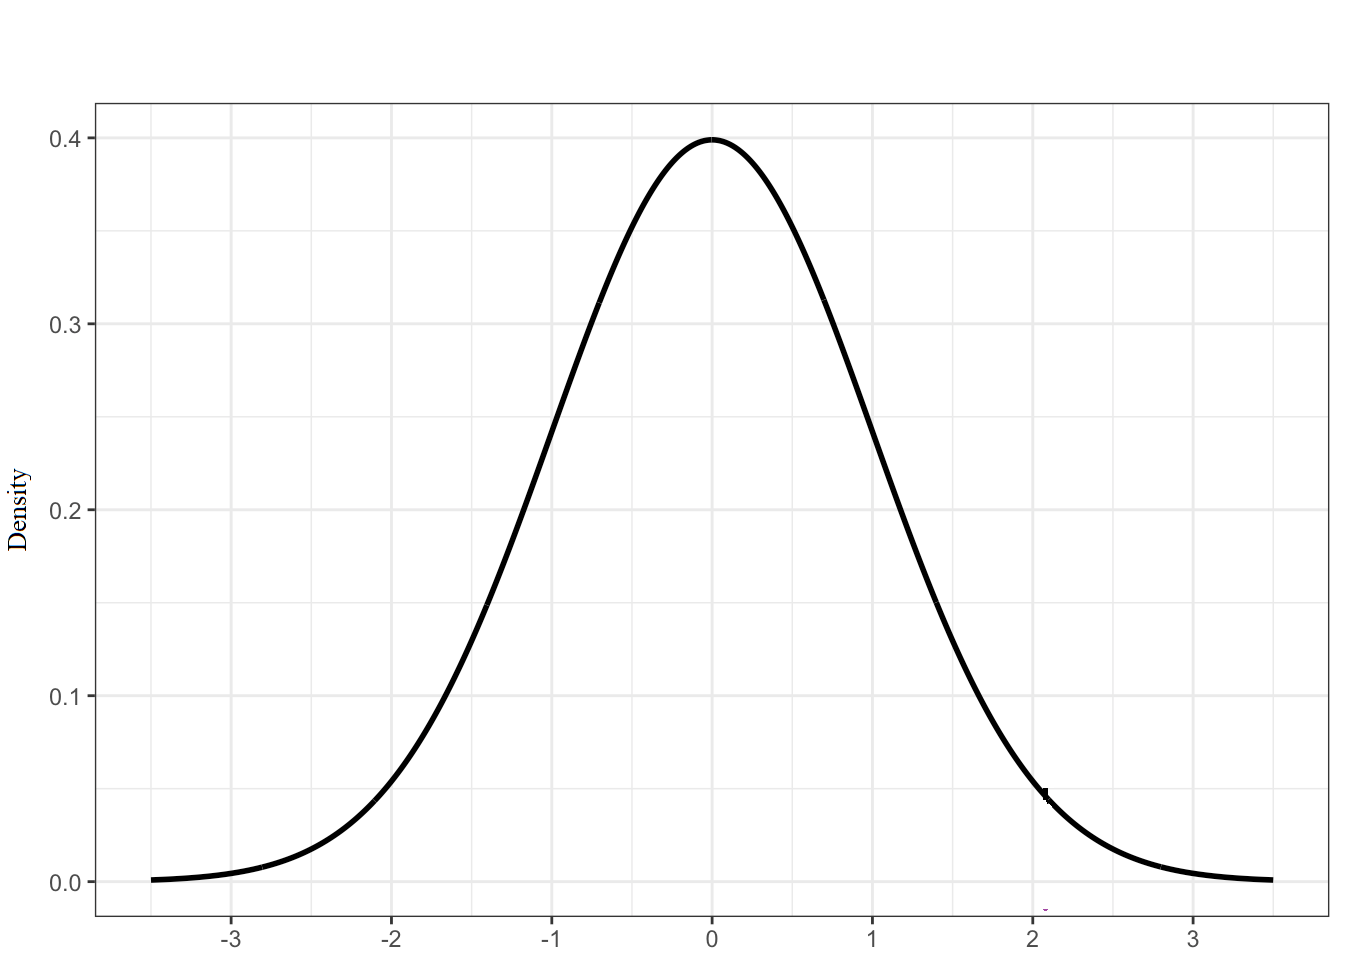
\includegraphics[scale=0.3]{pvalue1.png}
	\end{center}
	
\end{frame}

\begin{frame}{Illustration of P-Value Construction}
	
	
	\begin{center}
		Normalized realization of the random estimator
		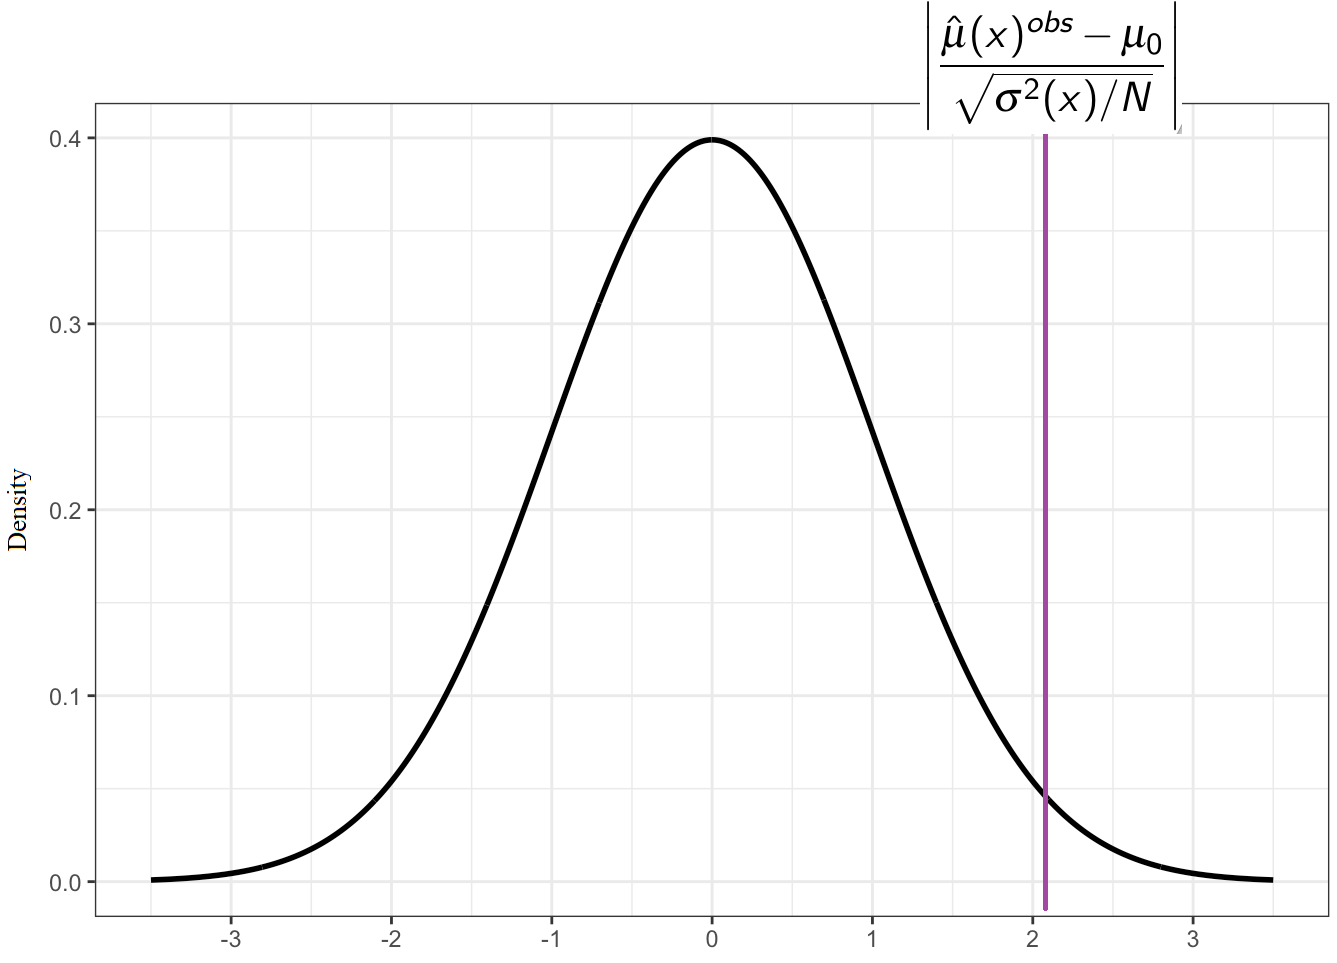
\includegraphics[scale=0.3]{pvalue2.png}
	\end{center}
	
\end{frame}

\begin{frame}{Illustration of P-Value Construction}		
	\begin{center}
		p-value calculation
		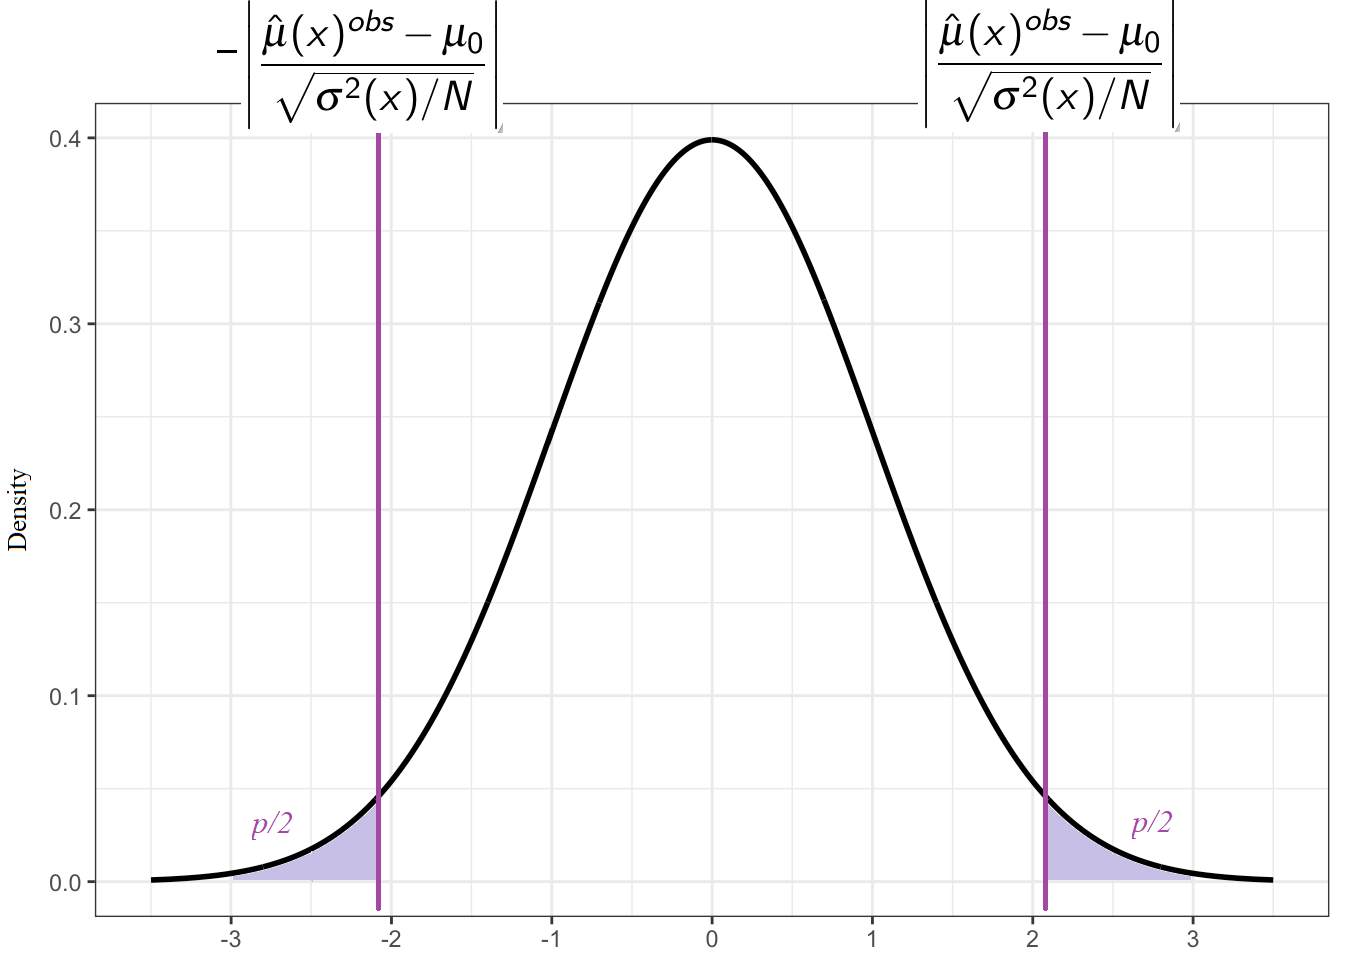
\includegraphics[scale=0.3]{pvalue3.png}
	\end{center}
\end{frame}




\begin{frame}{When Do We Reject the Null?}

\begin{wideitemize}
	\item 
	Recall that our $p$-value takes the form
	$$1 - \left(  \Phi(|\hat{t}|) - \Phi( -|\hat{t}| )  \right) $$
	
	\item
	It turns out that $\Phi(1.96) - \Phi(-1.96) \approx 0.95$. Thus, $p < 0.05$ if and only if $|\hat{t}| > 1.96$. So we reject at the 5\% level if $|\hat{t}| > 1.96$. 
	
	\pause
	\item
	What does this imply about the value of $\mu_0$ we reject/don't reject?
	
	\pause
	\item
	We don't reject if 	
	$$ |\hat{t}| \leq 1.96 \pause \implies \dfrac{ |\hat\mu - \mu_0| }{ \sigma / \sqrt{N} } \leq 1.96 \pause \implies \mu_0 \in  [\hat\mu - 1.96 \sigma / \sqrt{N} , \hat\mu + 1.96 \sigma \sqrt{N}]$$
\vspace{-0.5cm}
	\pause
	\item
	The interval $\hat\mu \pm 1.96 \sigma / \sqrt{N}$ is thus the 95\% confidence interval (CI)
	\smallskip

		\begin{itemize}
			\item 
			It has the property that $Pr( \mu_0 \in CI ) = 0.95$ when $H_0: \mu = \mu_0$ is true
		\end{itemize}
	
\end{wideitemize}
	
\end{frame}



\begin{frame}{Significance and Power}
	
	\begin{itemize}
		\item The \emph{significance level} (or \emph{size}) of a test is the pre-specified probability of incorrectly rejecting the null when it is true (type-I error rate)
		 \pause
		 \begin{itemize}
		 	\item 
		 	E.g. a 5\% level test rejects when $p<0.05$.
		 \end{itemize}
		\pause
		\bigskip

		\item The \emph{power} of a test is the probability of correctly rejecting the null when it is false (1 - type-II error rate)
		
			\begin{itemize}
				\item 
				The power is a function of the \textit{alternative} hypothesis. I.e., the probability that we reject $H_0:\mu=\mu_0$ when in fact $\mu = \mu_A$ 
			\end{itemize}
	\end{itemize}

\end{frame}




\begin{frame}{Caution about $P$-Value Interpretation}

\begin{itemize}
\item Frequentist p-values are often interpreted as ``probability that $H_0$ is true.'' Is this right? \pause{} No!


\begin{wideitemize}
	\item $p$-value tells us the probability of getting the observed data \emph{assuming} the null is true
	
	\item That is, $p$-value tells us about $P(data | H_0)$, not $P(H_0 | data)$. 

	\item By Bayes' rule, $P(H_0 | Data) = P(Data | H_0) * P(H_0) / P(Data)$. But to formalize this, we need to take a stand on our \emph{prior} belief that $H_0$ is true, $P(H_0)$. 
	
\end{wideitemize}


\pause
\bigskip
\item People often interpret a $p<0.05$ as strong evidence of an effect and $p \geq 0.05$ as evidence of no effect. 

	\begin{itemize}
		\item 
		But $p=0.05$ is a fairly arbitrary threshold. 
		\vspace{0.1cm}
		\item
		It's better to view the $p$-value as a spectrum indicating how likely is the observed data given the null.  \pause
		\vspace{0.1cm}
		\item
		Moreover, $p$-values can be large even if the null is false (low power!)
	\end{itemize}
\end{itemize}

\end{frame}

\begin{frame}

\begin{center}

\includegraphics[scale=0.45]{p-values0.jpg}
\end{center}

\end{frame}

\begin{frame}

\vspace{0.8cm}
\begin{center}

\includegraphics[scale=0.45]{p-values.jpg}
\end{center}

\end{frame}



\begin{frame}{What About Non-Normal Data?}
\vspace{0.2cm}
\begin{itemize}
\item So we know how to test hypotheses and make inferences on means of normal random variables when we know their variance ... so what?
\pause{}
\smallskip

\begin{itemize}
\item Most variables are not normally distributed!\pause{}
\vspace{0.1cm}
\item Even when they are, why would we know their variance?!\pause{}
\vspace{0.1cm}
\item Have I just been wasting your time!?! \pause{} No.\pause{}
\end{itemize}
\vspace{0.4cm}

\item We will next review powerful \textbf{asymptotic} results. These will allow us to apply similar inference tools if the sample is ``large'' even when $Y_i$ is not normally distributed.
\end{itemize}

\end{frame}

\end{document}
}
